% Name: Area under a curve
% Description: The definite integral of f from a to b, shaded under the curve.
% Tags: integral, area, definite integral

\usetikzlibrary{arrows.meta}

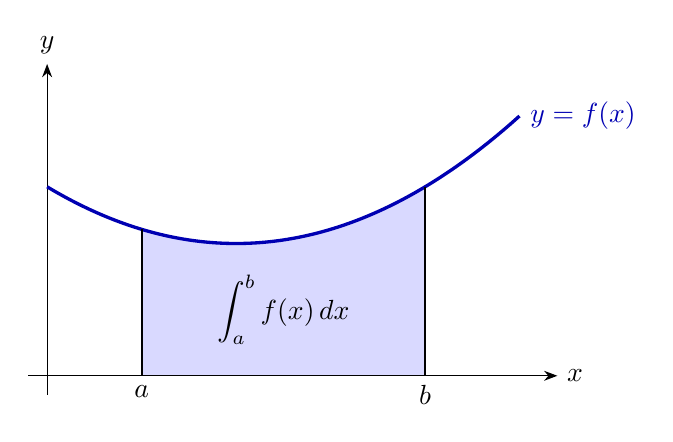
\begin{tikzpicture}[>={Stealth}, scale=1.2]
  \fill[blue!15] (1,0) -- plot[domain=1:4, samples=40] (\x, {0.15*\x*\x - 0.6*\x + 2}) -- (4,0) -- cycle;
  \draw[->] (-0.2,0) -- (5.4,0) node[right] {$x$};
  \draw[->] (0,-0.2) -- (0,3.3) node[above] {$y$};
  \draw[very thick, blue!70!black, domain=0:5, samples=60, smooth]
    plot (\x, {0.15*\x*\x - 0.6*\x + 2}) node[right] {$y = f(x)$};
  \draw[thick] (1,0) -- (1,1.55) (4,0) -- (4,2.0);
  \node[below] at (1,0) {$a$};
  \node[below] at (4,0) {$b$};
  \node at (2.5,0.7) {$\displaystyle\int_a^b f(x)\,dx$};
\end{tikzpicture}
